\begin{figure}[htp]
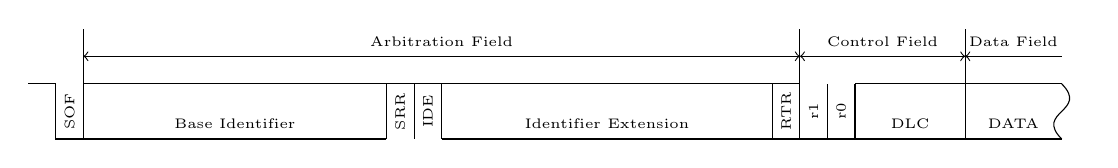
\begin{tikzpicture}[scale=0.7]
	%SOF
	\draw (0,1) -- ++(0.5,0) -- ++(0,-1) -- ++(0.5,0) -- ++(0,1);
	\node[rotate=90] at (0.75,0.5) {\tiny SOF};
	%Base Identifier
	\draw (1,1) -- ++(5.5, 0);
	\draw (1,0) -- ++(5.5, 0) node[midway, above=0.25] {\tiny Base Identifier};
	\draw (6.5, 0) -- ++(0,1);
	%SRR
	\draw (6.5, 1) -- ++(0.5,0);
	\draw (7, 0) -- ++(0,1);
	\node[rotate=90] at (6.75,0.5) {\tiny SRR};
	%IDE
	\draw (7, 1) -- ++(0.5,0);
	\draw (7.5, 0) -- ++(0,1);
	\node[rotate=90] at (7.25,0.5) {\tiny IDE};
	%Identifier Extension
	\draw (7.5,1) -- ++(6, 0);
	\draw (7.5,0) -- ++(6, 0) node[midway, above=0.25] {\tiny Identifier Extension};
	\draw (13.5, 0) -- ++(0,1);
	%RTR
	\draw (13.5,0) -- ++(0.5,0);
	\draw (13.5,1) -- ++(0.5,0);
	\draw (14,0) -- ++(0,1);
	\node[rotate=90] at (13.75,0.5) {\tiny RTR};
	%R1 R0
	\draw (14,0) -- ++(1,0);
	\draw (14.5,0) -- ++(0,1);
	\node[rotate=90] at (14.25,0.5) {\tiny r1};
	\draw (15,0) -- ++(0,1);
	\node[rotate=90] at (14.75,0.5) {\tiny r0};
	%DLC
	\draw (15,1) -- ++(2,0);
	\draw (15,0) -- ++(2,0) node[midway, above=0.25] {\tiny DLC};
	\draw (17, 0) -- ++(0,1);
	%Data
	\draw (17,1) -- ++(1.75,0);
	\draw (17,0) -- ++(1.75,0) node[midway, above=0.25] {\tiny DATA};
	\draw (18.75,0) .. controls (18.25,0.5) and (19.25,0.5) .. (18.75,1);
	
	%Arbitration
	\draw (1,1) -- ++(0,1);
	\draw (14,1) -- ++(0,1);
	\draw[<->] (1,1.5) -- (14,1.5) node[midway, above] {\tiny Arbitration Field};
	%Control
	\draw (17,1) -- ++(0,1);
	\draw[<->] (14,1.5) -- (17,1.5) node[midway, above] {\tiny Control Field};
	%Data
	\draw[<-] (17,1.5) -- ++(1.75,0) node[midway, above] {\tiny Data Field};
	
	\end{tikzpicture}
	\caption{CAN Extended Frame}
	\label{fig:can_ext_frame}
\end{figure}